%----------------------------------------------------------------------------------------
%	PACKAGES AND OTHER DOCUMENT CONFIGURATIONS
%----------------------------------------------------------------------------------------

\documentclass[paper=a4, fontsize=11pt]{scrartcl} % A4 paper and 11pt font size

\usepackage[T1]{fontenc} % Use 8-bit encoding that has 256 glyphs
\usepackage{fourier} % Use the Adobe Utopia font for the document - comment this line to return to the LaTeX default
%\usepackage{palatino}
\usepackage[english]{babel} % English language/hyphenation
\usepackage{amsmath,amsfonts,amsthm} % Math packages

\usepackage{enumerate}
\usepackage{listings}  % Use this for better code formatting
%\usepackage{amssymb}
%\usepackage{xcolor} 
\usepackage{graphicx}    
\usepackage[svgnames]{xcolor} 

%\usepackage{sectsty} % Allows customizing section commands
%\allsectionsfont{\centering \normalfont\scshape} % Make all sections centered, the default font and small caps
 \usepackage{setspace} 
 
\usepackage{fancyhdr} % Custom headers and footers
\pagestyle{fancyplain} % Makes all pages in the document conform to the custom headers and footers
\fancyhead{} % No page header - if you want one, create it in the same way as the footers below
\fancyfoot[L]{} % Empty left footer
\fancyfoot[C]{} % Empty center footer
\fancyfoot[R]{\thepage} % Page numbering for right footer
\renewcommand{\headrulewidth}{0pt} % Remove header underlines
\renewcommand{\footrulewidth}{0pt} % Remove footer underlines
\setlength{\headheight}{13.6pt} % Customize the height of the header
\setlength{\parindent}{0cm}
\setlength{\parskip}{.1cm plus4mm minus3mm}


%--- color definitions for code listings
\definecolor{mygreen}{rgb}{0,0.6,0}
\definecolor{mygray}{rgb}{0.5,0.5,0.5}
\definecolor{mymauve}{rgb}{0.58,0,0.82}


% commands I use to typeset matrices in bold
\newcommand{\matLambda}{\mathbf{\Lambda}}
\newcommand{\matSigma}{\mathbf{\Sigma}}
\newcommand{\vecBeta}{\mathbf{\beta}}
\newcommand{\vecC}{\mathbf{c}}
\newcommand{\vecEpsilon}{\mathbf{\epsilon}}
\newcommand{\vecMu}{\mathbf{\mu}}
\newcommand{\vecY}{\mathbf{y}}
\newcommand{\matA}{\mathbf{A}}
\newcommand{\matB}{\mathbf{B}}
\newcommand{\matC}{\mathbf{C}}
\newcommand{\matI}{\mathbf{I}}
\newcommand{\matP}{\mathbf{P}}
\newcommand{\matS}{\mathbf{S}}
\newcommand{\matV}{\mathbf{V}}
\newcommand{\matQ}{\mathbf{Q}}
\newcommand{\matX}{\mathbf{X}}
\newcommand{\matY}{\mathbf{Y}}
\newcommand{\matW}{\mathbf{W}}



%\numberwithin{equation}{section} % Number equations within sections (i.e. 1.1, 1.2, 2.1, 2.2 instead of 1, 2, 3, 4)
%\numberwithin{figure}{section} % Number figures within sections (i.e. 1.1, 1.2, 2.1, 2.2 instead of 1, 2, 3, 4)
%\numberwithin{table}{section} % Number tables within sections (i.e. 1.1, 1.2, 2.1, 2.2 instead of 1, 2, 3, 4)

%\setlength\parindent{0pt} % Removes all indentation from paragraphs - comment this line for an assignment with lots of text

%----------------------------------------------------------------------------------------
%	TITLE SECTION
%----------------------------------------------------------------------------------------

\newcommand{\horrule}[1]{\rule{\linewidth}{#1}} % Create horizontal rule command with 1 argument of height

\title{	
\normalfont \normalsize 
%\textsc{stat 8004} \\ [25pt] 
\horrule{0.5pt} \\[0.4cm] % Thin top horizontal rule
\huge STAT 8004, Assignment 4 \\ % The assignment title
\horrule{2pt} \\[0.5cm] % Thick bottom horizontal rule
}

\author{David Dobor} 

\date{\normalsize\today} % Today's date or a custom date

\lstset{ %
  language=R,                     % the language of the code
  basicstyle=\small\ttfamily,
  backgroundcolor=\color{WhiteSmoke},  % choose the background color. You must add \usepackage{color}
  showspaces=false,               % show spaces adding particular underscores
  showstringspaces=false,         % underline spaces within strings
  showtabs=false,                 % show tabs within strings adding particular underscores
  frame=single,                   % adds a frame around the code
  rulecolor=\color{Gray},        % if not set, the frame-color may be changed on line-breaks within not-black text (e.g. commens (green here))
  tabsize=2,                      % sets default tabsize to 2 spaces
  captionpos=b,                   % sets the caption-position to bottom
  breaklines=true,                % sets automatic line breaking
  breakatwhitespace=false,        % sets if automatic breaks should only happen at whitespace
  title=\lstname,                 % show the filename of files included with \lstinputlisting;
                                  % also try caption instead of title
  keywordstyle=\color{DarkSlateBlue},      % keyword style
  commentstyle=\color{ForestGreen},   % comment style
  stringstyle=\color{mymauve},      % string literal style
  %escapeinside={\%*}{*)},         % if you want to add a comment within your code
  morekeywords={*,det,...}            % if you want to add more keywords to the set
} 

\renewcommand{\ttdefault}{pcr}  %to be able to use bold fonts in lstlistings code

\begin{document}

\maketitle 

%----------------------------------------------------------------------------------------
%	PROBLEM 1
%----------------------------------------------------------------------------------------
\subsection*{Question 1}
In the context of Problem 2 of Homework Assignment 3, use \texttt{R} matrix 
calculations to do the following in the (non-full-rank) Gauss-Markov normal linear 
model


\begin{enumerate}[(a)]
\item Find 90\% two-sided confidence limits for $\sigma$.

\item Find 90\% two-sided confidence limits for $\mu + \tau_2$.

\item Find 90\% two-sided confidence limits for $\tau_1 -  \tau_2$.

\item Find a $p$-value for testing the null hypothesis $H_0 \ : \tau_1 -  \tau_2 = 0 \ $ vs $\ H_a \ : \text{ not } \ H_0$.

\item Find 90\% two-sided prediction limits for the sample mean of $ n = 10$ future observations from
the first set of conditions.

\item Find 90\% two-sided prediction limits for the difference between a pair of future values, one
from the first set of conditions (i.e. with mean  $\mu + \tau_1$ ) and one from the second set of conditions
(i.e. with mean  $\mu + \tau_2$).

\item Find a $p$-value for testing $H_0 \ : \ 
\begin{bmatrix} 0 & 1 & -1 & 0 & 0 \\
                             0 & 1 & 0 & -1 & 0 \\
                             0 & 1 & 0 & 0 & -1
\end{bmatrix}
\begin{bmatrix} \mu\\
                             \tau_1\\
                             \tau_2\\
                             \tau_3\\
                             \tau_4
\end{bmatrix}
=
\begin{bmatrix} 0\\
                             0\\
                             0
\end{bmatrix}
$. What is the practical interpretation of this test?

\item Find a $p$-value for testing $H_0 \ : \ 
\begin{bmatrix} 0 & 1 & -1 & 0 & 0 \\
                             0 & 0 & 1 & -1 & 0 \\
\end{bmatrix}
\begin{bmatrix} \mu\\
                             \tau_1\\
                             \tau_2\\
                             \tau_3\\
                             \tau_4
\end{bmatrix}
=
\begin{bmatrix} 10\\
                             0
\end{bmatrix}
$. 
\end{enumerate}
\bigskip
\subsubsection*{Answer to Question 1}
The context is the one-way \texttt{ANOVA} Gauss-Markov model  $y_{ij} = \mu + \tau_i + \epsilon_{ij}$ 
for the $j$th  individual of the $i$th group  (4 groups with sample sizes  2, 1, 1, 2 for groups, respectively)
as follows:
$$
\begin{bmatrix} 
2\\ 1\\ 4 \\ 6 \\ 3\\ 5  
\end{bmatrix}
=
\begin{bmatrix} 1 & 1 & 0 & 0 & 0 \\
                             1 & 1 & 0 & 0 & 0 \\
                             1 & 0 & 1 & 0 & 0\\
                             1 & 0 & 0 & 1 & 0 \\
                             1 & 0 & 0 & 0 & 1\\
                             1 & 0 & 0 & 0 & 1
\end{bmatrix}
\begin{bmatrix} 
\mu \\ \tau_1\\ \tau_2 \\ \tau_3 \\ \tau_4 \\ 
\end{bmatrix}
+ 
\begin{bmatrix} 
\epsilon_{1 1 } \\ \epsilon_{1 2}\\ \epsilon_{2 1} \\ \epsilon_{3 1} \\ \epsilon_{4 1} \\\epsilon_{42}  
\end{bmatrix}
$$
%----------------------------------------------------------------------------------------
%	ANSWER TO PROBLEM 1
%----------------------------------------------------------------------------------------
\begin{enumerate}[(a)]
\item With $n = 6$ observations and the design matrix being of rank 4, we find that 

$$\frac{\text{SSE}}{ \sigma^2}  \sim \chi^2_{n - \text{rank(X)}} = \chi^2_{2}.$$
That is
$$
P \left(\frac{\text{SSE}}{\text{upper  0.05 } \text{qt of }\chi^2_{2} }  <  \sigma^2 < \frac{\text{SSE}}{\text{lower  0.05 } \text{qt of }\chi^2_{2}}  \right) = 0.9.
$$\\
\begin{lstlisting}[basicstyle=\ttfamily\small\bfseries]
# compute sum of squared errors
beta.hat <- ginv(t(X) %*% X) %*% t(X) %*% Y
Y.hat <- X %*% beta.hat;  
SSE <- t(Y - Y.hat) %*% (Y - Y.hat) # ans: 2.5

# compute the endpoints for the 90% confidence interval
lower.limit <- SSE / qchisq(0.95, 2)  # ans: 0.4172603
upper.limit <- SSE / qchisq(0.05, 2)  # ans: 24.36966

c(sqrt(lower.limit), sqrt(upper.limit))
#ans: 0.6459568 4.9365633
\end{lstlisting}
The 90\% confidence interval for $\sigma$ is given by:
\boxed{
$$
\left( 0.6459\ , \ 4.9366\right)
$$
}\\

\pagebreak

\item  Here $c^T = (1, 0, 1, 0, 0)$ (we have $c^T \vecBeta = \mu + \tau_2$). We note that 
 $c^T \vecBeta$ is an estimable function ($c^T$ is the third row of $X$) and compute the
 two sided 90\% confidence interval as follows:\\
 
 \begin{lstlisting}[basicstyle=\ttfamily\small\bfseries]
c <- matrix(c(1, 0, 1, 0, 0), 5, 1)
c.beta.hat <- t(c) %*% beta.hat #= 4
MSE <- SSE / df

# 90% two sided confidence interval
c.beta.hat +
    c(-1, 1) * qt(.95, df)* sqrt(MSE) * sqrt(t(c) %*% XtXi %*% c)
#ans: 0.7353569 7.2646431
\end{lstlisting}

 The 90\% confidence interval for $\mu + \tau_2$ is given by:
\boxed{
$$
\left( 0.7353569\ , \  7.2646431\right)
$$
}\\
 \\
 

\item  Here $c^T = (0, 1, -1, 0, 0)$ (we have $c^T \vecBeta = \tau_1 - \tau_2$). We note that 
 $c^T \vecBeta$ is an estimable function ($c^T$ is ( row 2 - row 3 ) of $X$  ) and compute the
 two sided 90\% confidence interval as follows:\\
 
 \begin{lstlisting}[basicstyle=\ttfamily\small\bfseries]
c <- matrix(c(0, 1, -1, 0, 0), 5, 1)
c.beta.hat <- t(c) %*% beta.hat #= -2.5

# 90% two sided confidence interval
c.beta.hat +
    c(-1, 1) * qt(.95, df) * sqrt(MSE) * sqrt(t(c) %*% XtXi %*% c)
#ans: -6.498355  1.498355
\end{lstlisting}

 The 90\% confidence interval for $\tau_1 - \tau_2$ is given by:
\boxed{
$$
\left(-6.498355\ , \  1.498355\right)
$$
}\\
 \\
 
 
 
\item Here
$$
H_0 \ : \ 
\begin{bmatrix} 0 & 1 & -1 & 0 & 0 
\end{bmatrix}
\begin{bmatrix} \mu\\
                             \tau_1\\
                             \tau_2\\
                             \tau_3\\
                             \tau_4
\end{bmatrix}
= \ 0
$$ 
And we compute the following $F$ ratio
$$
F = \frac{\text{SSH}_0 \ / 1 }{ \text{SSE }  / \ 2 } = \frac{\text{MSH}_0 }{ \text{MSE } } 
$$
as follows:
 \begin{lstlisting}[basicstyle=\ttfamily\small\bfseries]
# here c and c.beta.hat are the same as in part (c)
# sum of squares under the null (numerator in the F test):
SSH <- 
    t(c.beta.hat) %*% ginv( (t(c) %*% XtXi %*% c) ) %*% c.beta.hat

SSE <- t(Y - Y.hat) %*% (Y - Y.hat)
MSH <- SSH
MSE <- SSE / df

# the F ratio
F <- MSH / MSE
# the p-value
1 - pf(F, 1, 2) #ans: 0.2094306

### alternatively, we could use this: 
t.stat <- c.beta.hat / (sqrt(MSE) * sqrt(t(c) %*% XtXi %*% c))
p.value <- 2*(1 - pt(abs(t.stat),df))
###
# the p.value is the same as with the F-test
###
\end{lstlisting}

The $p$-value here is \ \fbox{0.2094306}\\


\item Following the notation used in class, for 10 future observations from the first set of conditions 
we set $c^T$ to be the first row of $X: \ \vecC^T = (1, 1, 0, 0, 0)$ (thus $\vecC^T \vecBeta$ is 
clearly estimable), and set $\gamma = 1/10$.  Then var$(y^*) = 1/10$. \\

Thus 
$$
\widehat{\vecC^T \vecBeta} - y^* \sim  N \left( 0, \sigma^2 (\gamma + \sigma^2\vecC^T (\matX^T \matX)^- \vecC) \right)
$$

independently of SSE. 






The $t$-test is then as follows:\\

 \begin{lstlisting}[basicstyle=\ttfamily\small\bfseries]
c <- matrix(c(1, 1, 0, 0, 0), 5, 1)
c.beta.hat <- t(c) %*% beta.hat #= 1.5
gamma <- 1/10
MSE <- SSE / df

c.beta.hat + c(-1,1) * qt(.95, df) * sqrt(MSE) *sqrt(gamma + t(c) %*% XtXi %*% c)

# ans: -1.028782  4.028782
\end{lstlisting}

Thus the 90\% two-sided prediction limits for the sample mean of $10$ future observations from
the first set of conditions are \fbox{(-1.028782,  4.028782)} \ . \\



\item For the difference of 2 future values we set $\gamma = 2$ and $\vecC^T = (2, 1, 1, 0, 0)$. The rest
is similar to part (e), as follows:\\
 \begin{lstlisting}[basicstyle=\ttfamily\small\bfseries]
c <- matrix(c(2, 1, 1, 0, 0), 5, 1)
c.beta.hat <- t(c) %*% beta.hat #= 5.5
gamma <- 2
MSE <- SSE / df

c.beta.hat + c(-1,1) * qt(.95, df) * sqrt(MSE) *sqrt(gamma + t(c) %*% XtXi %*% c)
# ans: -0.607588 11.607588
\end{lstlisting}

Thus the 90\% two-sided prediction limits for the difference between a pair of future values, one
from the first set of conditions (i.e. with mean  $\mu + \tau_1$ ) and one from the second set of conditions
(i.e. with mean  $\mu + \tau_2$) are \fbox{(-0.607588,  11.607588)} \ . \\


\item The practical interpretation here is that the effects for groups 2, 3, and 4 (the values $\tau_1, \tau_2, \tau_3$) are not that different 
from the effect for group 1 (from the value of $\tau_1$). \\

Parts (g) and (h) are similar to (d). Results follow in this \texttt{R} code:\\
 \begin{lstlisting}[basicstyle=\ttfamily\small\bfseries]
C <- t(matrix(c(0, 1, -1, 0, 0,
                0, 1, 0, -1, 0,
                0, 1, 0, 0, -1), nrow=5, ncol=3))
C.beta.hat <- C %*% beta.hat
# sum of squares under the null (numerator in the F test):
SSH <-
    t(C.beta.hat) %*% ginv( (C %*% XtXi %*% t(C)) ) %*% C.beta.hat
MSH <- SSH / 3

SSE <- t(Y - Y.hat) %*% (Y - Y.hat)
MSE <- SSE / df
# the F ratio
F <- MSH / MSE
1 - pf(F, 1, 2) #ans: 0.1835034
\end{lstlisting}

The $p$-value is \ \fbox{0.1835034}\\


\item   
 
 \begin{lstlisting}[basicstyle=\ttfamily\small\bfseries]
C <- t(matrix(c(0, 1, -1, 0, 0,
                0, 0, 1, -1, 0), nrow=5, ncol=2))
d <- matrix(c(10,0))
u <- C %*% beta.hat - d
# sum of squares under the null (numerator in the F test):
SSH <-
    t(u) %*% ginv( (C %*% XtXi %*% t(C)) ) %*% u
SSE <- t(Y - Y.hat) %*% (Y - Y.hat)
MSH <- SSH /2 
MSE <- SSE / df
# the F ratio
F <- MSH / MSE
1 - pf(F, 1, 2) #ans: 0.01329846
\end{lstlisting}

The $p$-value is \ \fbox{ 0.01329846}\\
\end{enumerate}

\bigskip
\bigskip
%----------------------------------------------------------------------------------------
%	PROBLEM 2
%----------------------------------------------------------------------------------------
\subsection*{Question 2}
In the following, make use of the data in Problem 4 of Homework Assignment 3. 
Consider a regression of $y$ on $x_1, x_2, \ldots, x_5$. Use \texttt{R} matrix 
calculation to do the following in a full rank Gauss-Markov normal linear model.\\



\begin{enumerate}[(a)]

\item Find 90\% two-sided confidence limits for $\sigma$.\\

\item Find 90\% two-sided confidence limits for the mean response under the conditions of data point \#1.\\

\item Find 90\% two-sided confidence limits for the difference in mean responses under the conditions
of data points \#1 and \#2.\\

\item Find a $p$-value for testing the hypothesis that the conditions of data points \#1 and \#2 produce
the same mean response.\\

\item Find 90\% two-sided prediction limits for an additional response for the set of conditions
$x_1 = 0.005, x_2 = 0.45, x_3 =7, x_4 = 45,$ and $x_5 = 6.$\\

\item Find a $p$-value for testing the hypothesis that a model including only $ x_1, x_3$ and $x_5$ is 
adequate for ``explaining'' home price. (Hint: write it in the form of $ H_0 \ : \matC \vecBeta = 0$).\\
\end{enumerate}
\bigskip
%----------------------------------------------------------------------------------------
%	ANSWER TO PROBLEM 2
%----------------------------------------------------------------------------------------
\subsubsection*{Answer to Question 2}

\begin{enumerate}[(a)]

\item The \texttt{Boston} dataset contains $n = 506$ observations. Also, rank($X$) = 6. So
$$\frac{\text{SSE}}{ \sigma^2}  \sim \chi^2_{n - \text{rank(X)}} = \chi^2_{500}.$$
That is
$$
P \left(\frac{\text{SSE}}{\text{upper  0.05 } \text{qt of }\chi^2_{500} }  <  \sigma^2 < \frac{\text{SSE}}{\text{lower  0.05 } \text{qt of }\chi^2_{500}}  \right) = 0.9.
$$\\

\begin{lstlisting}[basicstyle=\ttfamily\small\bfseries]
# after loading the data as in assignment 3, we do:
# compute sum of squared errors
beta.hat <- ginv(t(X) %*% X) %*% t(X) %*% Y
Y.hat <- X %*% beta.hat;  
SSE <- t(Y - Y.hat) %*% (Y - Y.hat) # ans: 17411.94

# compute the endpoints for the 90% confidence interval
lower.limit <- SSE / qchisq(0.95, 500)  # ans: 31.4791
upper.limit <- SSE / qchisq(0.05, 500)  # ans: 38.7667
\end{lstlisting}
Thus the 90\% confidence interval for $\sigma$ is:
$$
\left(\sqrt{31.4791},  \ \sqrt{38.7667}\right)  \\
$$
\begin{center}
\boxed{
$$
\left(5.610624,  \ 6.226291\right)  
$$
}\\
\end{center}
\pagebreak



\item 

\begin{lstlisting}[basicstyle=\ttfamily\small\bfseries]
c <- X[1,]   # data point # 1: first row
c.beta.hat <- t(c) %*% beta.hat # ans: 25.70437

# 90% two sided confidence interval
c.beta.hat +
    c(-1, 1) * qt(.95, df)* sqrt(MSE) * sqrt(t(c) %*% XtXi %*% c)

# ans: 25.21142 26.19733
\end{lstlisting}

Answer to (b):
\begin{center}
\boxed{
$$
\left(25.21142,  \ 26.19733\right) 
$$
}\\
\end{center}
\vspace{5mm}

\item
\begin{lstlisting}[basicstyle=\ttfamily\small\bfseries]
c <- X[1,] - X[2,]   # data point # 1: first row - second row
c.beta.hat <- t(c) %*% beta.hat #

# 90% two sided confidence interval
c.beta.hat +
    c(-1, 1) * qt(.95, df)* sqrt(MSE) * sqrt(t(c) %*% XtXi %*% c)

# ans: 1.202479 2.612541
\end{lstlisting}

Answer to (c):
\begin{center}
\boxed{
$$
\left(1.202479,  \ 2.612541\right) 
$$
}\\
\end{center}
\vspace{5mm}

\item
\begin{lstlisting}[basicstyle=\ttfamily\small\bfseries]
# here c and c.beta.hat are the same as in part (c)
c <- X[1,] - X[2,]   # data point # 1: first row - second row
c.beta.hat <- t(c) %*% beta.hat 

# two sided t-test
p.value <- 2*(1 - pt(abs(c.beta.hat / (sqrt(MSE) * sqrt(t(c) %*% XtXi %*% c))),df))
# ans: 1.019758e-05
\end{lstlisting}

Answer to (d):
\begin{center}
\boxed{
$$0.00001019758$$
}\\
\end{center}

\vspace{5mm}


\item
\begin{lstlisting}[basicstyle=\ttfamily\small\bfseries]
c <- c(1, 0.005, 0.45, 7, 45, 6)
se <- sqrt(MSE)*sqrt(1 + c %*% XtXi %*% c)   #ans: 5.917394
c.beta.hat <- t(c) %*% beta.hat 

c.beta.hat + c(-1, 1) * qt(.95, df) * se
# ans: 19.90023 39.40286
\end{lstlisting}

Answer to (e):
\begin{center}
\boxed{
\left(19.90023,  \ 39.40286\right) 
}\\
\end{center}

\vspace{5mm}


% part (g)
\item 
We interpret the hypothesis  ``a model including only $ x_1, x_3$ and $x_5$ is 
adequate for explaining home price'' as $H_0 \ : \beta_2 = \beta_4 = 0$ and 
write  $H_0$  in the form $\matC \vecBeta = 0$:  
$$  
\begin{bmatrix} 0 & 0 & 1 & 0 & 0 & 0\\
                             0 & 0 & 0 & 0 & 1 & 0
\end{bmatrix}
\begin{bmatrix} \beta_0\\
                             \beta_1\\
                             \beta_2\\
                             \beta_3\\
                             \beta_4 \\
                             \beta_5
\end{bmatrix}
=
\begin{bmatrix} 0\\
                             0
\end{bmatrix}
$$  
We have that the following ratio is $F$ distributed
$$
F = \frac{\text{SSH}_0 \  / \  2}{ \text{SSE }  / \  500 }
$$

\begin{lstlisting}[basicstyle=\ttfamily\small\bfseries]
C <- matrix( 
    c(0, 0, 
      0, 0, 
      1, 0,
      0, 0, 
      0, 1,
      0, 0),
    nrow=2, 
    ncol=6) 

XtXi <- ginv(t(X) %*% X); 
C.beta.hat <- C %*% beta.hat

# sum of squares under the null (numerator in the F test):
SSH <- 
    t(C.beta.hat) %*% ginv( (C %*% XtXi %*% t(C)) )  %*% C.beta.hat

# squared errors (same as before, part (a) denominator in the F test):
SSE <- t(Y - Y.hat) %*% (Y - Y.hat) # ans: 17411.94
MSE <- SSE / df

# the F-ratio and the p-value
F <- (SSH / 2) / MSE
1 - pf(F, 2, 500)   #ans: 3.190781e-13
\end{lstlisting}

Thus the $p$-value is negligeable (3.190781e-13). 

(this tiny $p$-value somehow doesn't sit well with me. Perhaps I've tested the wrong hypothesis) 

\end{enumerate}
\bigskip
\bigskip
%----------------------------------------------------------------------------------------
%	PROBLEM 3
%----------------------------------------------------------------------------------------
\subsection*{Question 3} 
\begin{enumerate}[(a)]
\item In the context of Problem 1, part (g), suppose that in fact $\tau_1 = \tau_2, \tau_3 = \tau_4 = \tau_1 - d\sigma$. What is the distribution of the $F$ statistic?\\
 
\item Use \texttt{R} to plot the power of an $\alpha = 0.05$ level test as a function of $d$ for $d \in [-5, 5]$, that is plotting $P(F > \text{the cut-off value})$ against $d$.  The \texttt{R} function \texttt{pf(q, df1, df2, ncp)} will compute cumulative (non-central) $F$ probabilities for you corresponding to the value \texttt{q}, for degrees of
freedom \texttt{df1} and \texttt{df2} when the non-centrality parameter is \texttt{ncp}.
\end{enumerate}

\bigskip
\subsubsection*{Answer to Question 3}
Given that
$$
\begin{bmatrix} 0 & 1 & -1 & 0 & 0 \\
                             0 & 1 & 0 & -1 & 0 \\
                             0 & 1 & 0 & 0 & -1
\end{bmatrix}
\begin{bmatrix} \mu\\
                             \tau_1\\
                             \tau_2\\
                             \tau_3\\
                             \tau_4
\end{bmatrix}
=
\begin{bmatrix} 0\\
                              d\sigma\\
                             d \sigma
\end{bmatrix}
$$

We will have a non-central $F$ distribution with 3 and 2 degrees of freedom (numerator of the $F$-ratio has a $\chi^2$ distribution with 3 degrees of freedom; denominator has 2). We compute the non-centrality parameter based on the following quantities.  

$$
(\matC (\matX^T \matX ) \matC^T)^{-1} = 
\begin{bmatrix} 5/6 & -1/6& -1/3 \\
                             -1/6 & 5/6 & -1/3 \\
                             -1/3& -1/2 & 4/3
\end{bmatrix}
$$


\begin{align*}
\frac{1}{\sigma^2}(\matC \vecBeta - d)^T (\matC (\matX^T \matX ) \matC^T)^{-1}  (\matC \vecBeta - d) = \frac{1}{\sigma^2} \sigma^2 d^2 \frac{3}{2}\\
\end{align*}
Then \emph{(reading the textbook would make one think that using 1/2 of this paramter would be the way to go. However, I'm following the lecture notes here)}:\\
\begin{center}
\boxed{
$$
\text{non-centrality parameter}=    \frac{3}{2} d^2
$$
}\\
\end{center}

\vspace{5mm}
\begin{enumerate}[(a)]

\item The distribution is the non-central $F$ with parameters $(3, 2, \frac{3}{2} d^2)$

\item The following \texttt{R} code produces the graph shown below:
\begin{lstlisting}[basicstyle=\ttfamily\small\bfseries]
d <- seq(-5,5,.1)
power <- 1-pf(qf(0.95, 3, 2), 3, 2, (3/2)*d^2)

library(ggplot2)
qplot(d, power, geom="line", 
      main="Power Calculations at the 0.05 Significance Level\n",
      xlab="paramter d")

ggsave(file="power.png")
\end{lstlisting}

\begin{center}
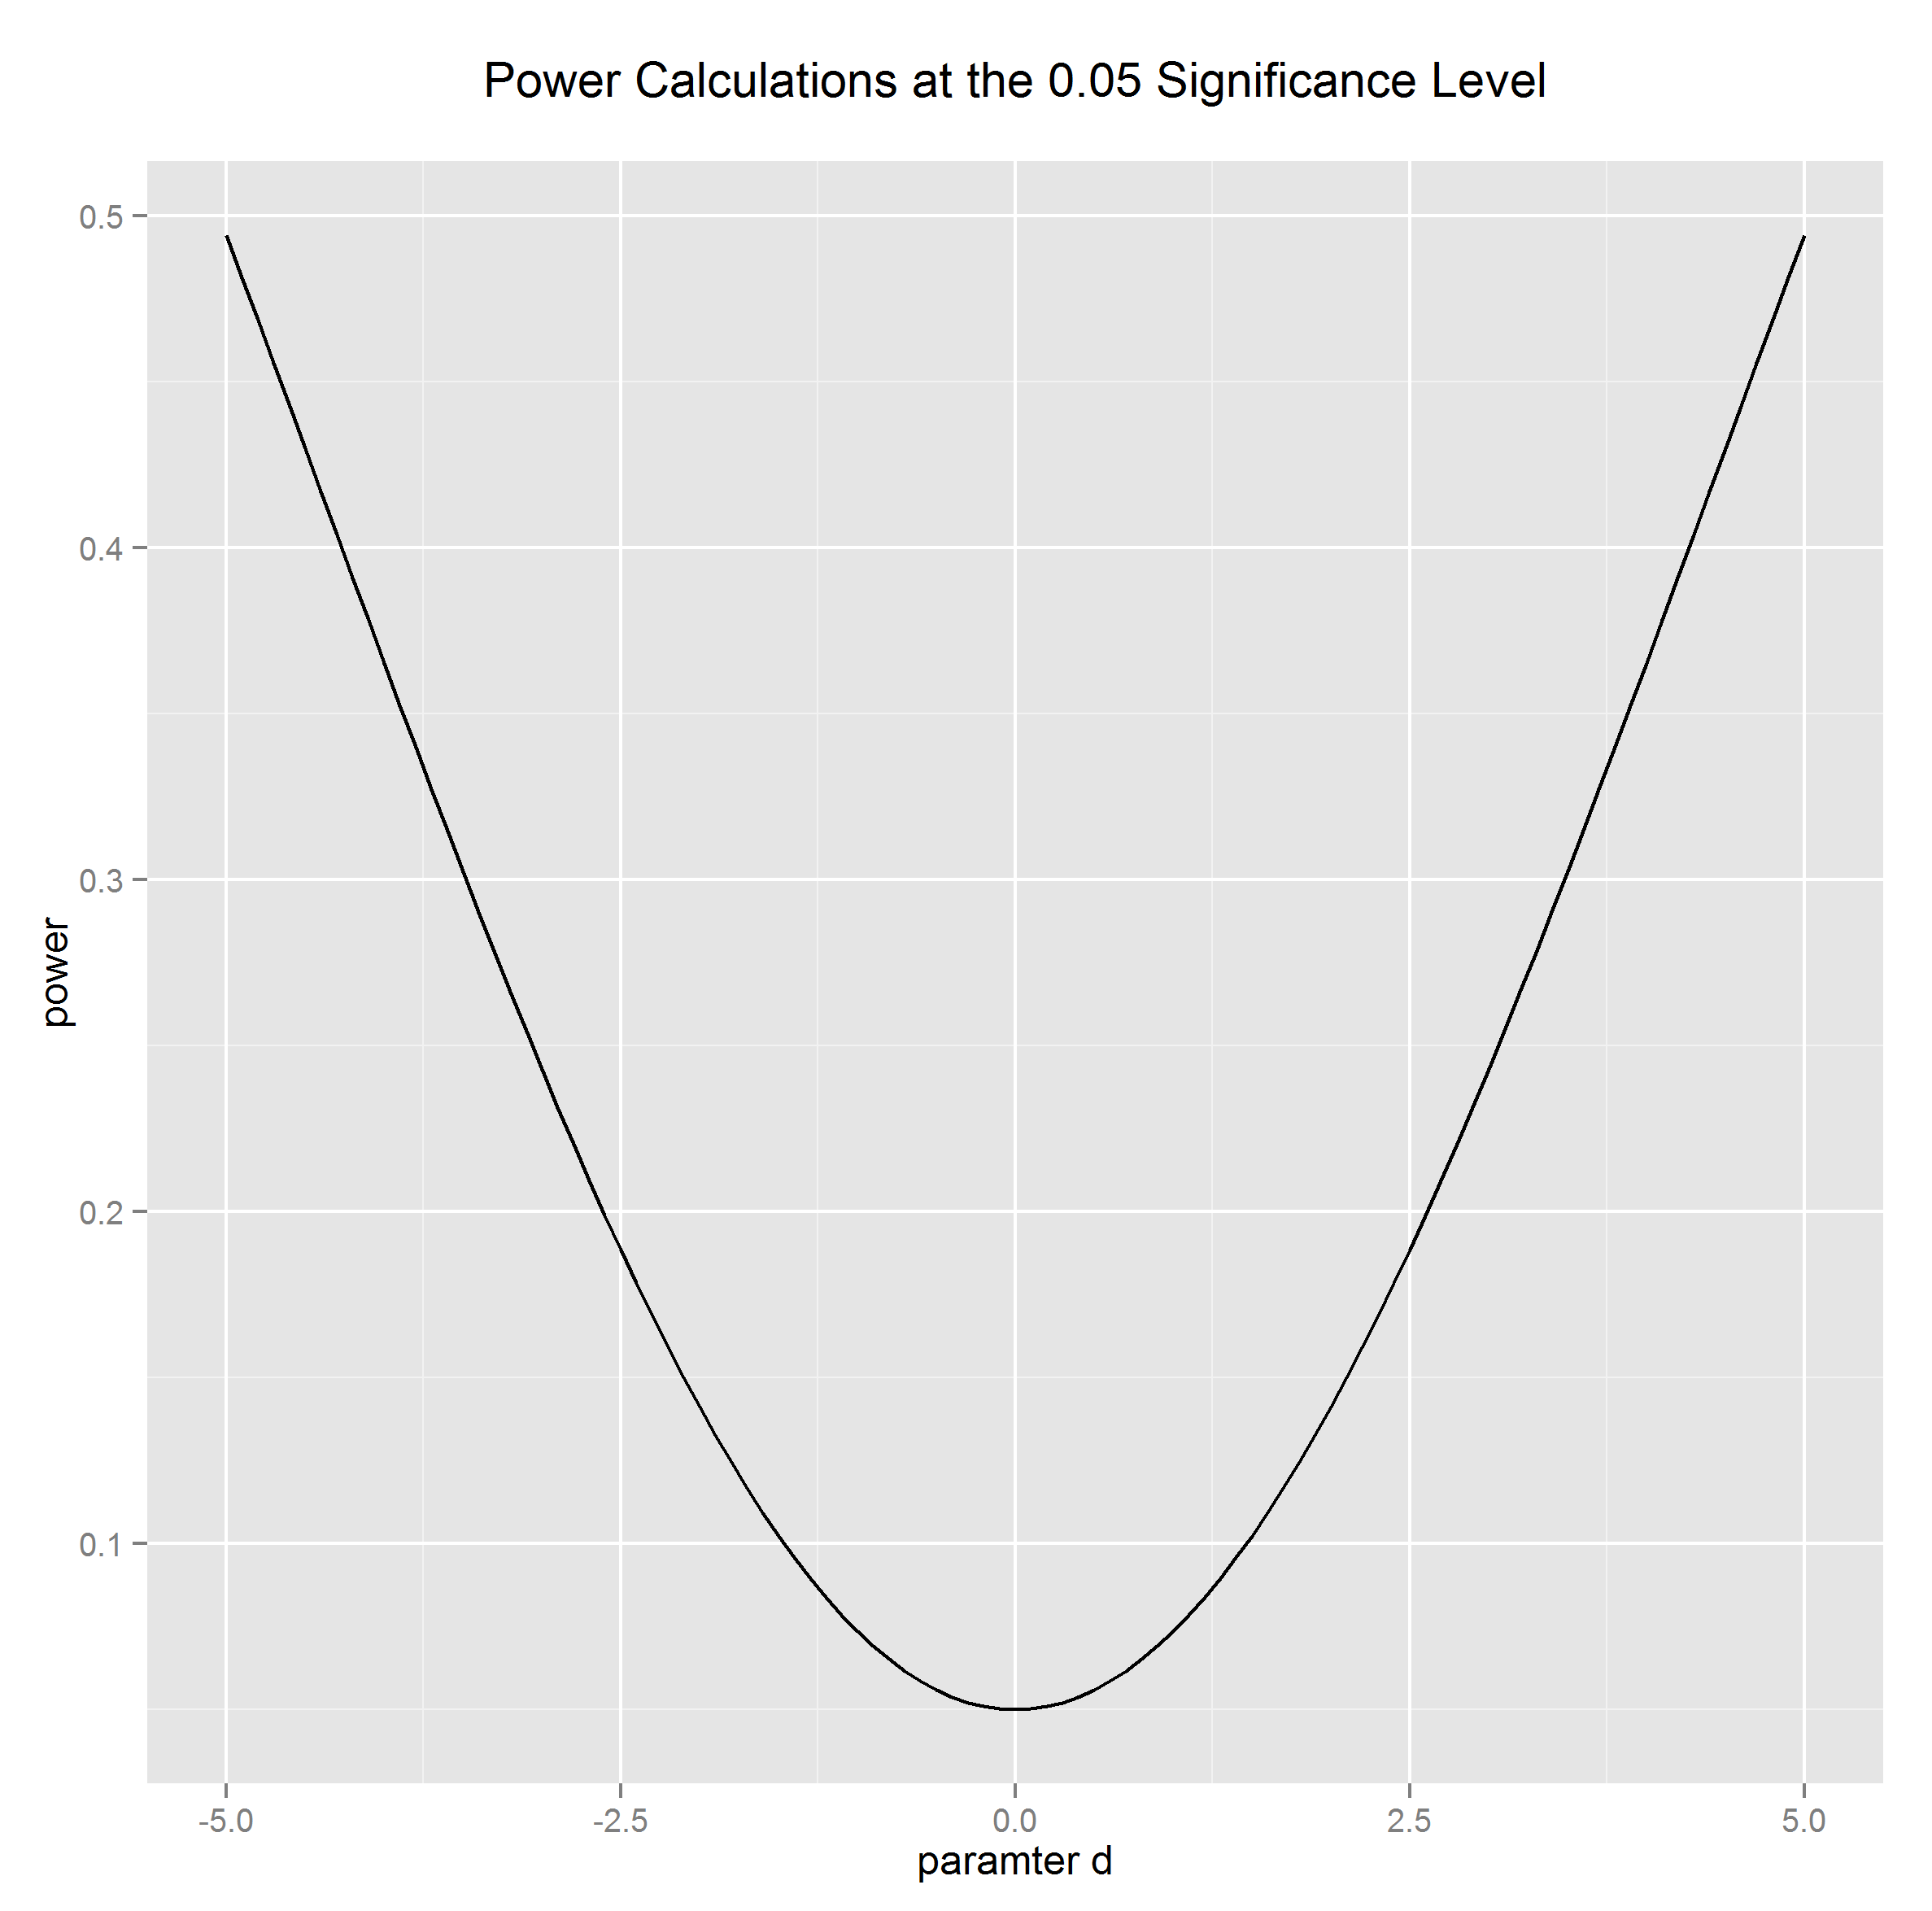
\includegraphics[width=10cm, height=12cm, width= 12cm]{power}
\end{center} 

\end{enumerate}


\pagebreak
\section*{Appendix}

Code used to obtain results for this assignment follows.\\

\begin{lstlisting}[basicstyle=\ttfamily\small\bfseries]
# question 1
library(MASS)

# data given for problem 2, previous assignment
X <- matrix( 
    c(1, 1, 1, 1, 1, 1, 
      1, 1, 0, 0, 0, 0,
      0, 0, 1, 0, 0, 0,
      0, 0, 0, 1, 0, 0, 
      0, 0, 0, 0, 1, 1 ), 
    nrow=6, 
    ncol=5) 

Y <- matrix(c(2, 1, 4, 6, 3, 5), 6, 1)


# compute some useful quantities used later
XtXi <- ginv(t(X) %*% X) 
n = 6 
df = n - qr(X)$rank  #degrees of freedom (used in tests below)
beta.hat <- XtXi %*% t(X) %*% Y
Y.hat <- X %*% beta.hat; 
SSE <- t(Y - Y.hat) %*% (Y - Y.hat) # ans: 2.5


#------------------------- part (a) -------------------------
# compute the endpoints for the 90% confidence interval
lower.limit <- SSE / qchisq(0.95, 2)  # ans: 0.4172603
upper.limit <- SSE / qchisq(0.05, 2)  # ans: 24.36966

c(sqrt(lower.limit), sqrt(upper.limit))
#ans: 0.6459568 4.9365633


#------------------------- part (b) -------------------------
c <- matrix(c(1, 0, 1, 0, 0), 5, 1)
c.beta.hat <- t(c) %*% beta.hat #= 4
MSE <- SSE / df

# 90% two sided confidence interval
c.beta.hat +
    c(-1, 1) * qt(.95, df)* sqrt(MSE) * sqrt(t(c) %*% XtXi %*% c)
#ans: 0.7353569 7.2646431


#------------------------- part (c) -------------------------
c <- matrix(c(0, 1, -1, 0, 0), 5, 1)
c.beta.hat <- t(c) %*% beta.hat #= -2.5

# 90% two sided confidence interval
c.beta.hat +
    c(-1, 1) * qt(.95, df) * sqrt(MSE) * sqrt(t(c) %*% XtXi %*% c)
#ans: -6.498355  1.498355


#------------------------- part (d) -------------------------
# here c and c.beta.hat are the same as in part (c)
# sum of squares under the null (numerator in the F test):
SSH <- 
    t(c.beta.hat) %*% ginv( (t(c) %*% XtXi %*% c) ) %*% c.beta.hat

SSE <- t(Y - Y.hat) %*% (Y - Y.hat)
MSH <- SSH
MSE <- SSE / df

# the F ratio
F <- MSH / MSE
# the p-value
1 - pf(F, 1, 2) #ans: 0.2094306

### alternatively, we could use this: 
t.stat <- c.beta.hat / (sqrt(MSE) * sqrt(t(c) %*% XtXi %*% c))
p.value <- 2*(1 - pt(abs(t.stat),df))
###
# the p.value is the same as with the F-test
###
#------------------------- part (e) -------------------------
c <- matrix(c(1, 1, 0, 0, 0), 5, 1)
c.beta.hat <- t(c) %*% beta.hat #= 1.5
gamma <- 1/10
MSE <- SSE / df

c.beta.hat + c(-1,1) * qt(.95, df) * sqrt(MSE) *sqrt(gamma + t(c) %*% XtXi %*% c)
# ans: -1.028782  4.028782


#------------------------- part (f) -------------------------
c <- matrix(c(2, 1, 1, 0, 0), 5, 1)
c.beta.hat <- t(c) %*% beta.hat #= 5.5
gamma <- 2
MSE <- SSE / df

c.beta.hat + c(-1,1) * qt(.95, df) * sqrt(MSE) *sqrt(gamma + t(c) %*% XtXi %*% c)
# ans: -0.607588 11.607588

#------------------------- part (g) -------------------------
C <- t(matrix(c(0, 1, -1, 0, 0,
                0, 1, 0, -1, 0,
                0, 1, 0, 0, -1), nrow=5, ncol=3))
C.beta.hat <- C %*% beta.hat
# sum of squares under the null (numerator in the F test):
SSH <-
    t(C.beta.hat) %*% ginv( (C %*% XtXi %*% t(C)) ) %*% C.beta.hat
MSH <- SSH / 3

SSE <- t(Y - Y.hat) %*% (Y - Y.hat)
MSE <- SSE / df
# the F ratio
F <- MSH / MSE
1 - pf(F, 1, 2) #ans: 0.1835034



#------------------------- part (h) -------------------------
C <- t(matrix(c(0, 1, -1, 0, 0,
                0, 0, 1, -1, 0), nrow=5, ncol=2))
d <- matrix(c(10,0))
u <- C %*% beta.hat - d
# sum of squares under the null (numerator in the F test):
SSH <-
    t(u) %*% ginv( (C %*% XtXi %*% t(C)) ) %*% u
SSE <- t(Y - Y.hat) %*% (Y - Y.hat)
MSH <- SSH /2 
MSE <- SSE / df
# the F ratio
F <- MSH / MSE
1 - pf(F, 1, 2) #ans: 0.01329846
\end{lstlisting}

\pagebreak


\begin{lstlisting}[basicstyle=\ttfamily\small\bfseries]
# assignment 4, problem 2
library(MASS)
data(Boston)

Y=as.matrix(Boston$medv)
X=as.matrix(Boston[,c('crim','nox','rm','age','dis')])
X=cbind(rep(1,dim(Boston)[1]),X)

# some preliminary quantities useful in what follows:
XtXi <- ginv(t(X) %*% X) 
n <- dim(X)[1]         # 506 observations
df <- n - qr(X)$rank   # 500 degrees of freedom
beta.hat <- XtXi %*% t(X) %*% Y
Y.hat <- X %*% beta.hat; 
SSE <- t(Y - Y.hat) %*% (Y - Y.hat)  # ans: 17411.94
MSE <- SSE / df                      # ans: 34.82387

#------------------------- part (a) -------------------------
# compute the endpoints for the 90% confidence interval
lower.limit <- SSE / qchisq(0.95, 500)  # ans: 31.4791
upper.limit <- SSE / qchisq(0.05, 500)  # ans: 38.7667

c(sqrt(lower.limit), sqrt(upper.limit))
# ans: 5.610624 6.226291

#------------------------- part (b) -------------------------
c <- X[1,]   # data point # 1: first row
c.beta.hat <- t(c) %*% beta.hat # ans: 25.70437

# 90% two sided confidence interval
c.beta.hat +
    c(-1, 1) * qt(.95, df)* sqrt(MSE) * sqrt(t(c) %*% XtXi %*% c)

# ans: 25.21142 26.19733


#------------------------- part (c) -------------------------
c <- X[1,] - X[2,]   # data point # 1: first row - second row
c.beta.hat <- t(c) %*% beta.hat #

# 90% two sided confidence interval
c.beta.hat +
    c(-1, 1) * qt(.95, df)* sqrt(MSE) * sqrt(t(c) %*% XtXi %*% c)

# ans: 1.202479 2.612541


#------------------------- part (d) -------------------------
# here c and c.beta.hat are the same as in part (c)
c <- X[1,] - X[2,]   # data point # 1: first row - second row
c.beta.hat <- t(c) %*% beta.hat 

# two sided t-test
p.value <- 2*(1 - pt(abs(c.beta.hat / (sqrt(MSE) * sqrt(t(c) %*% XtXi %*% c))),df))
# ans: 1.019758e-05


#------------------------- part (e) -------------------------
c <- c(1, 0.005, 0.45, 7, 45, 6)
se <- sqrt(MSE)*sqrt(1 + c %*% XtXi %*% c)   #ans: 5.917394
c.beta.hat <- t(c) %*% beta.hat 

c.beta.hat + c(-1, 1) * qt(.95, df) * se
# ans: 19.90023 39.40286


#------------------------- part (f) -------------------------
C <- matrix( 
    c(0, 0, 
      0, 0, 
      1, 0,
      0, 0, 
      0, 1,
      0, 0),
    nrow=2, 
    ncol=6) 

XtXi <- ginv(t(X) %*% X); 
C.beta.hat <- C %*% beta.hat

# sum of squares under the null (numerator in the F test):
SSH <- 
    t(C.beta.hat) %*% ginv( (C %*% XtXi %*% t(C)) )  %*% C.beta.hat

# squared errors (same as before, part (a) denominator in the F test):
SSE <- t(Y - Y.hat) %*% (Y - Y.hat) # ans: 17411.94
MSE <- SSE / df

# the F-ratio and the p-value
F <- (SSH / 2) / MSE
1 - pf(F, 2, 500)   #ans: 3.190781e-13
\end{lstlisting}




\end{document}